\section{Durchführung}
\label{sec:Durchführung}

\subsection{Aufbau}
Der Aufbau dieses Versuchs ist recht simpel; es gibt 2 Stäbe (runder und eckiger
Grundfläche), welche horizontal an einer Apparatur befestigt werden, sodass
2 am oberen Teil der Apparatur befestigten Messuhren auf dem Stab aufliegen.
Sie dienen dazu, eine vertikale Deformierung im Milimeter-Bereich zu dokumentieren.
Zunächst wird ein Stab einseitig befestigt, das geschieht als erstes ohne,
dann mit Gewicht. Es ist wichtig, dass eine Nullmessung durchgeführt wird, da 
die Stäbe selbst ohne explizite Kraftzuführung durch Gravitation ausgelenkt werden.
In den folgenden Abbildungen ist der Aufbau für den beschriebenen Versuch jeweils 
mit Gewicht dargestellt. \\
\\
\\
\\
\\
\\
\\
\\
\begin{figure}[h]
    \centering
    \begin{minipage}{0.45\textwidth}
        \centering
        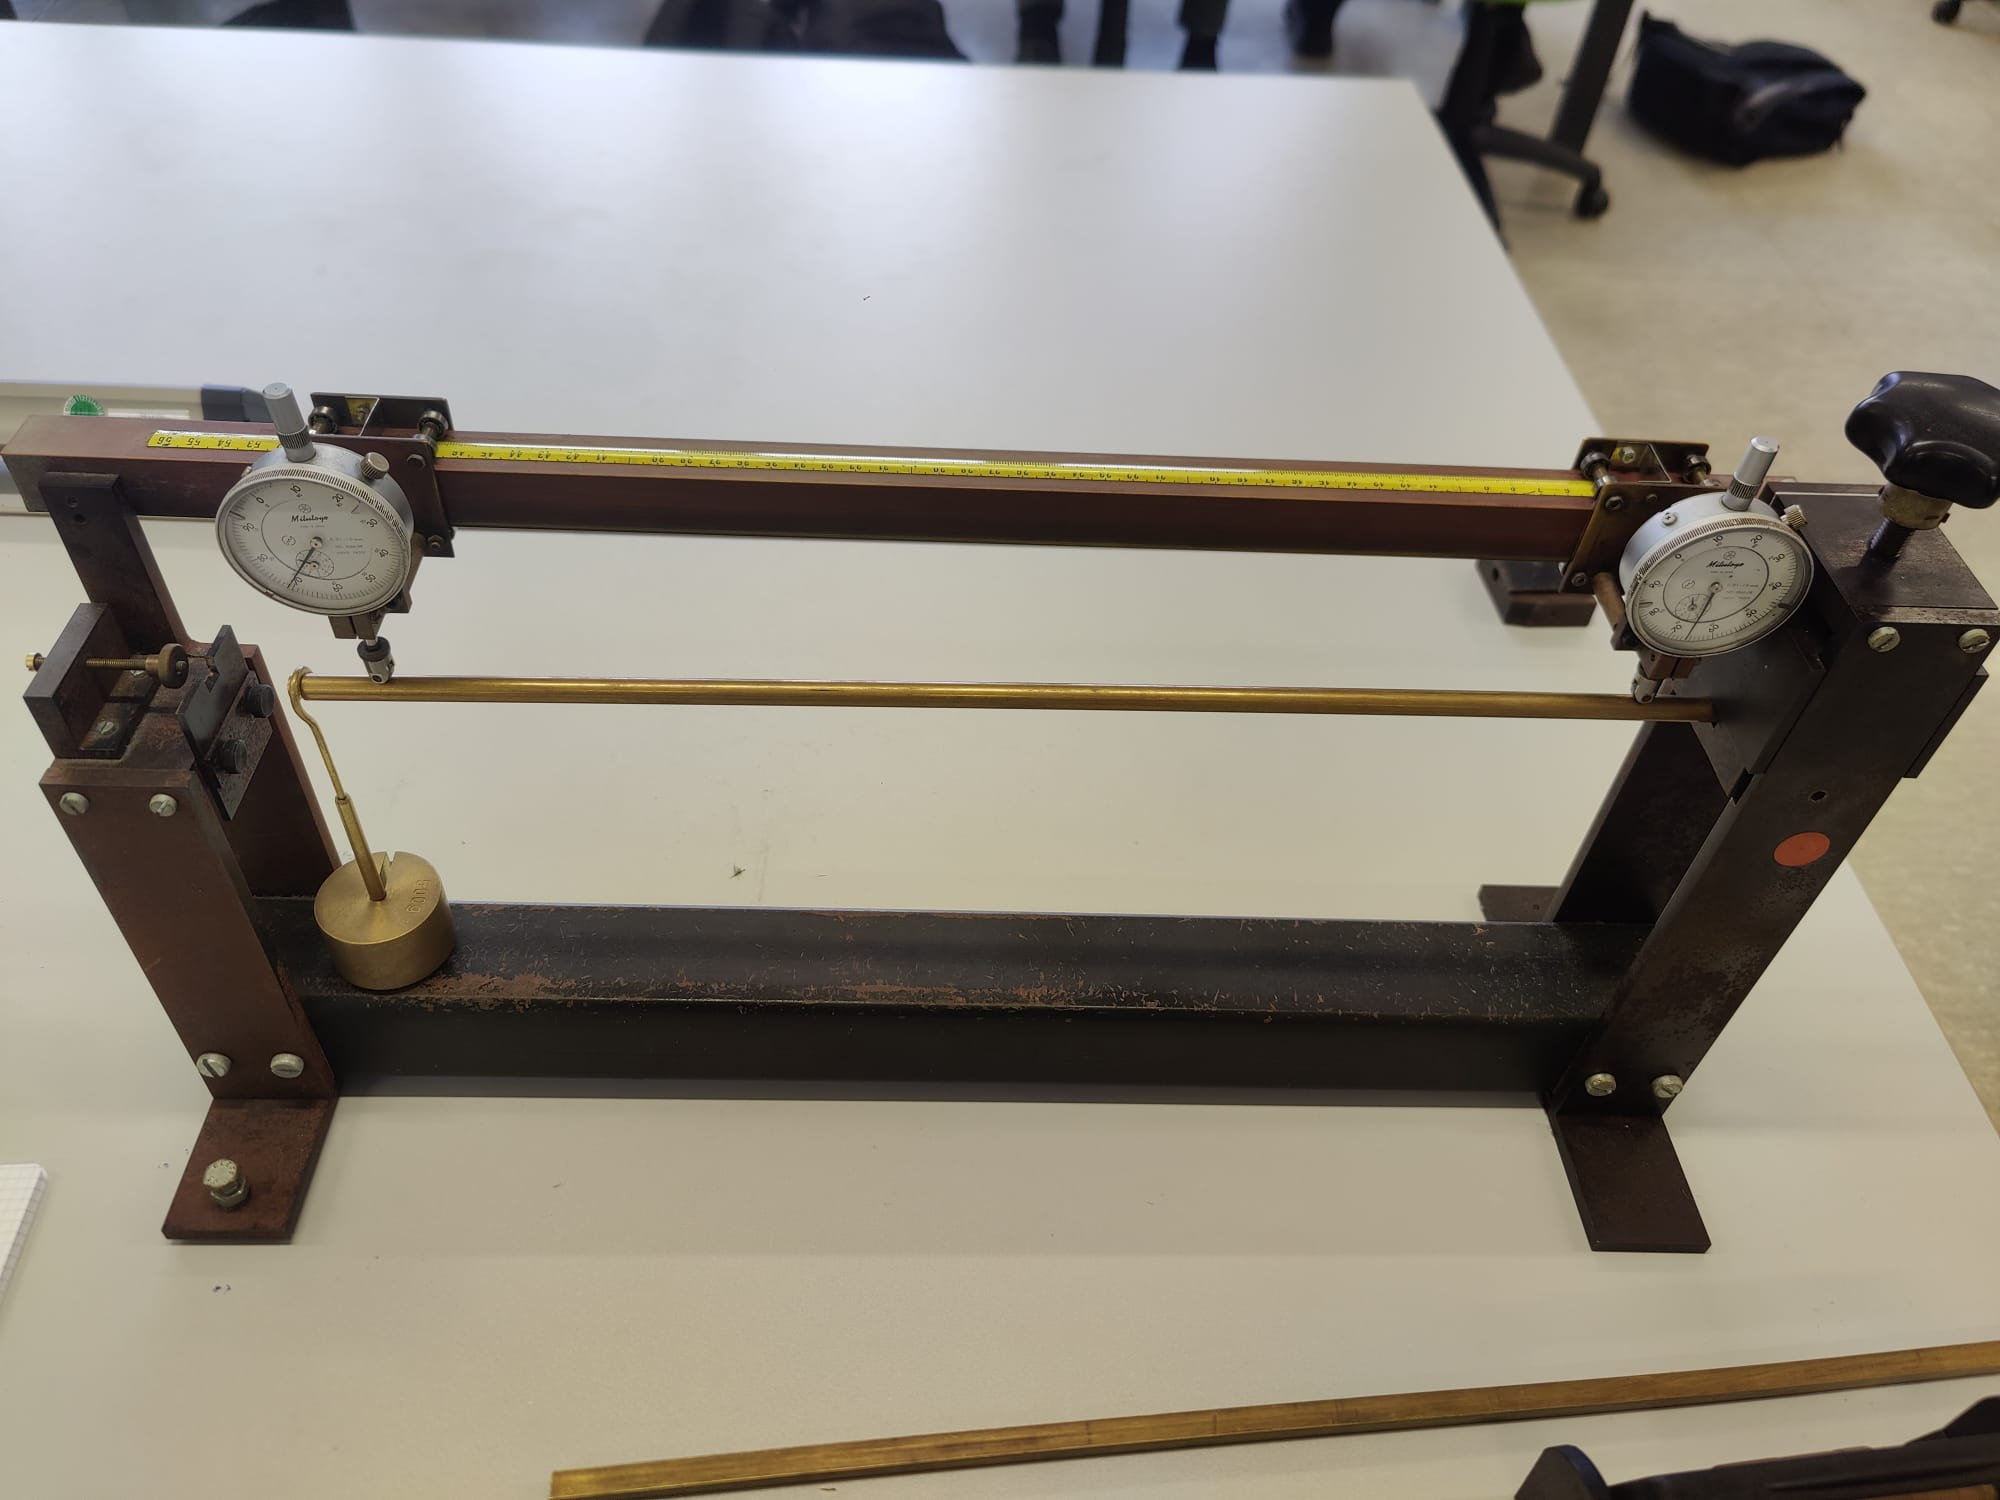
\includegraphics[width=\textwidth]{Bilder/emG2.jpg}
        \caption{Einseitige Einspannung des \\ runden Stabs mit Gewicht}
    \end{minipage}
    \hfill
    \begin{minipage}{0.45\textwidth}
        \centering
        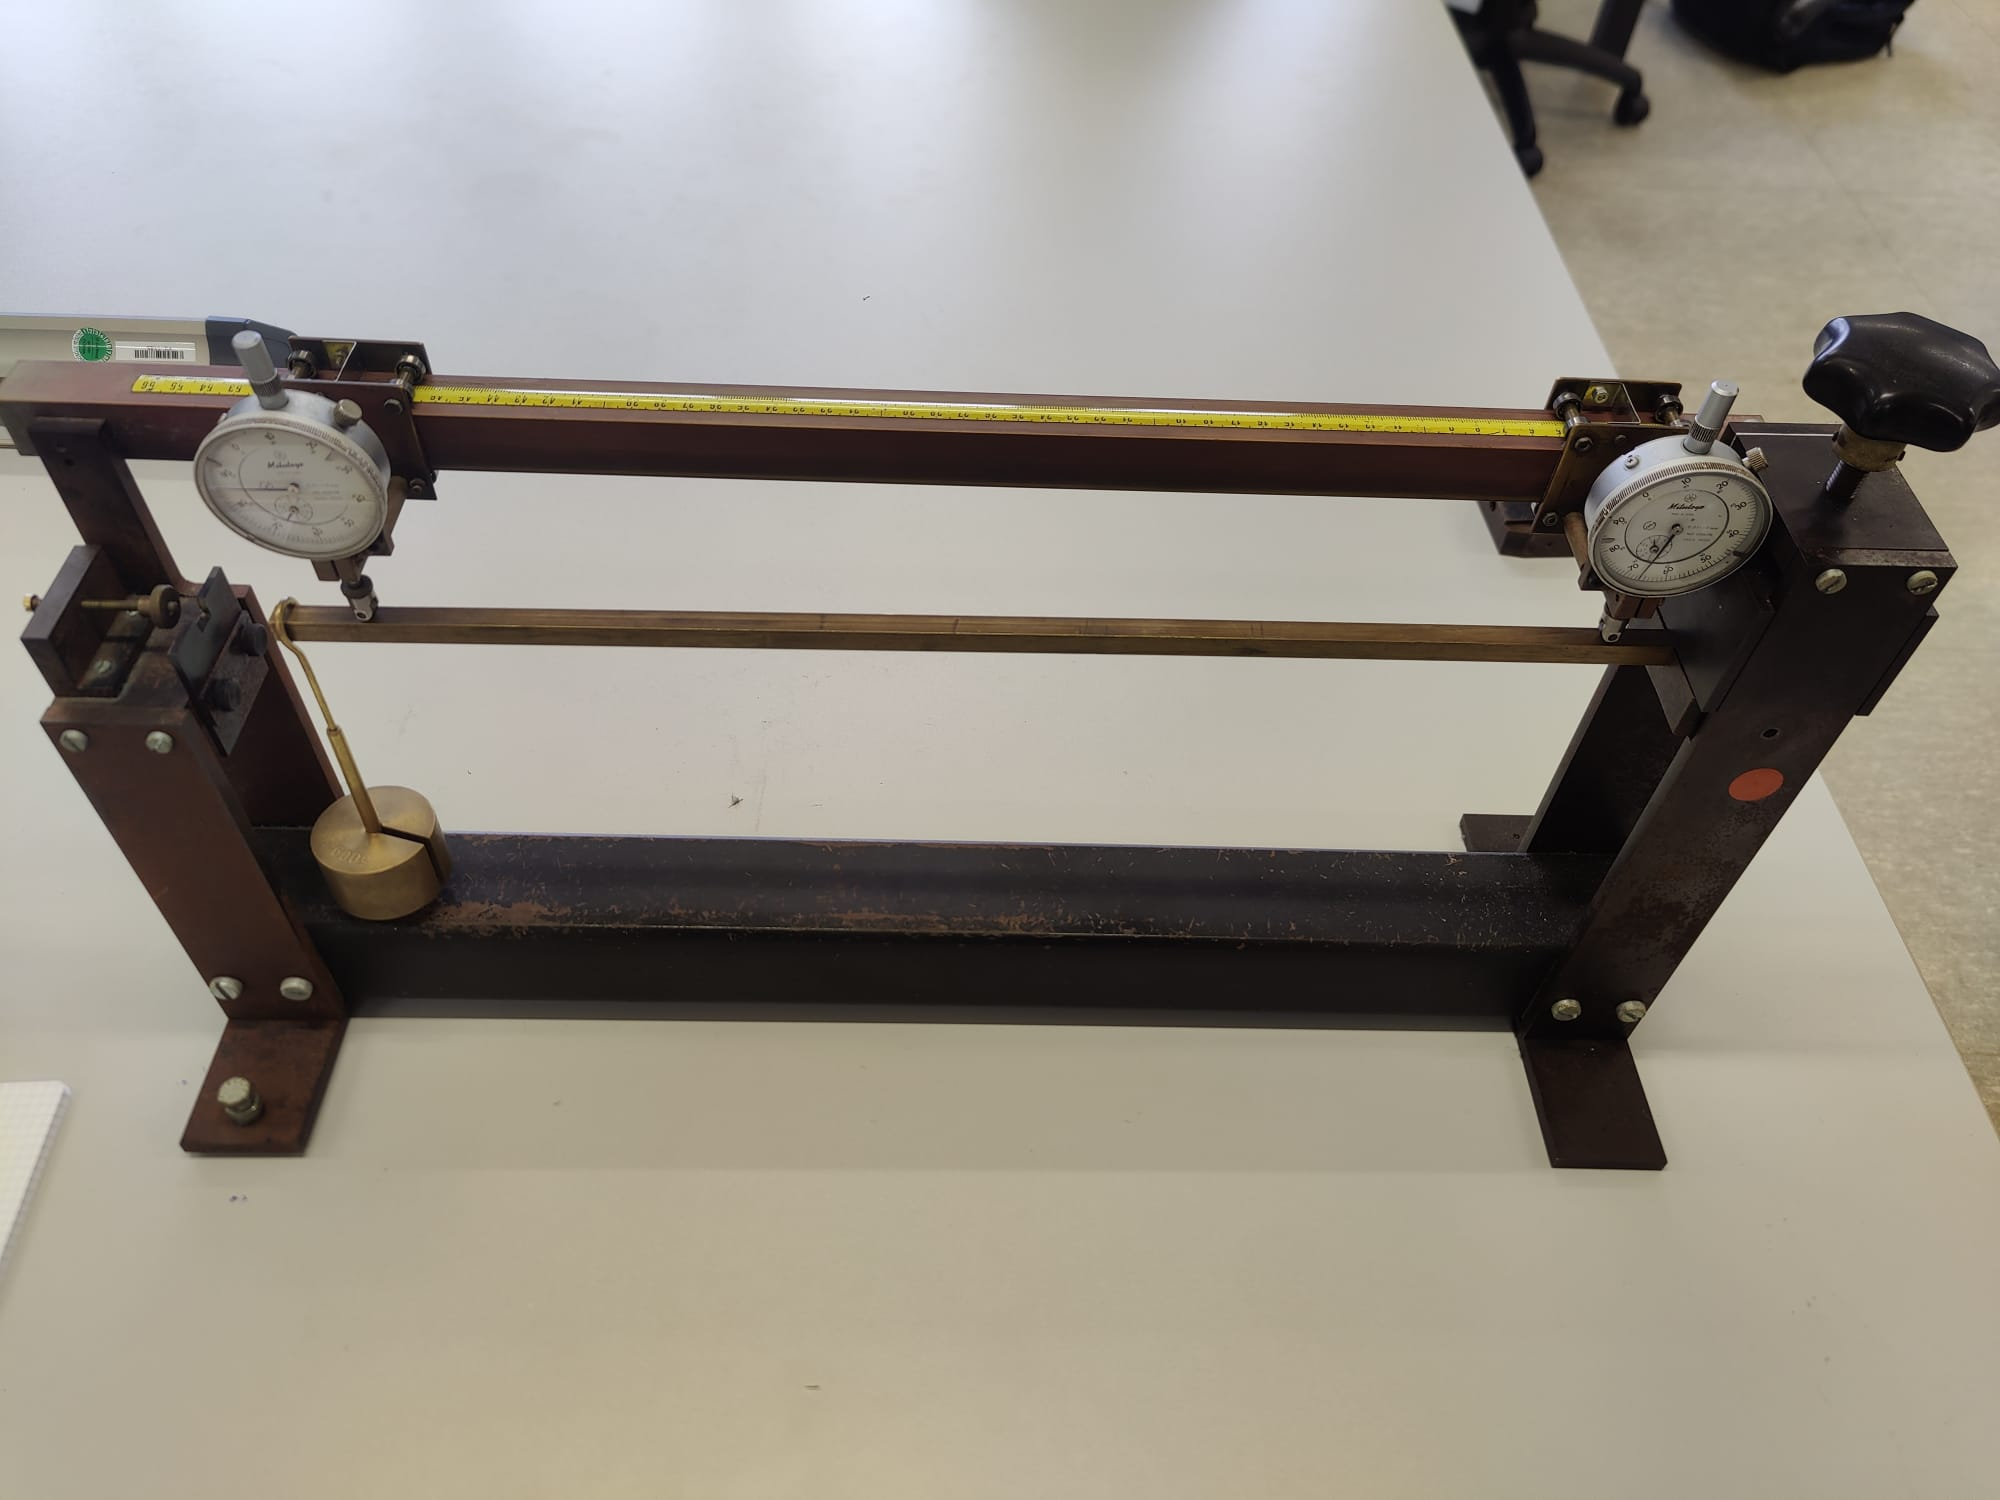
\includegraphics[width=\textwidth]{Bilder/emG.jpg}
        \caption{Einseitige Einspannung des \\ eckigen Stabs mit Gewicht}
    \end{minipage}
\end{figure}
Analog erfolgt der Versuch für eine beidseitige Befestigung; Der Stab mit und 
ohne Gewicht wird an der Apparatur befestigt, sodass die Uhren aufliegen. Das 
Gewicht sollte genau mittig sein, so bleiben die Fehler bei Messungen gering.
\begin{figure}[h]
    \centering
    \begin{minipage}{0.45\textwidth}
        \centering
        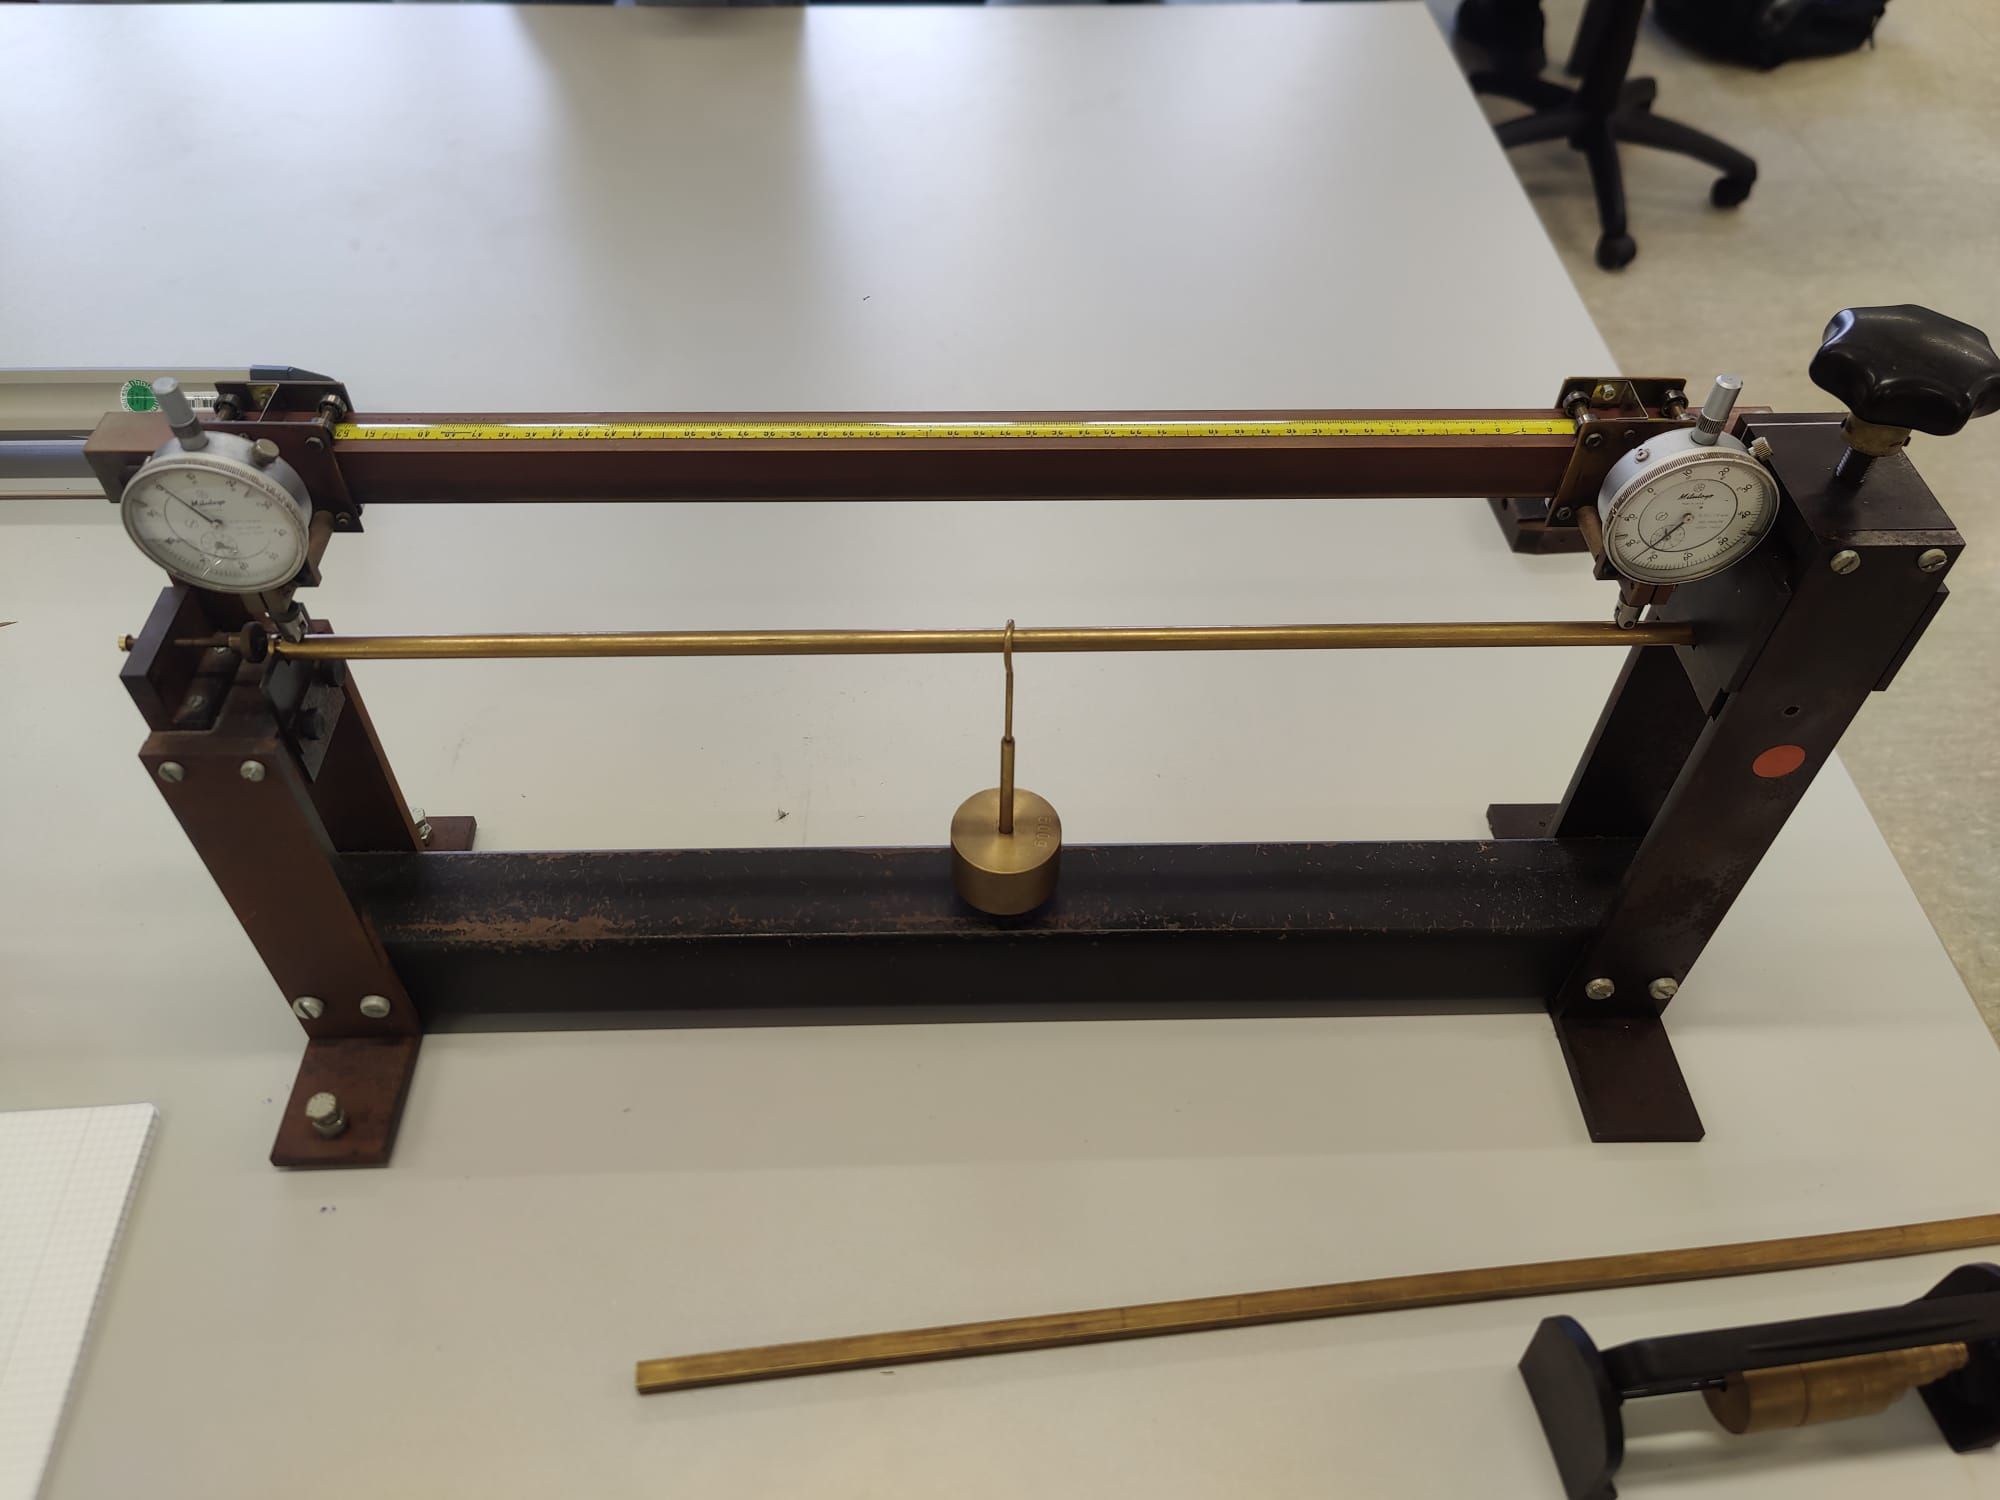
\includegraphics[width=\textwidth]{Bilder/bmG.jpg}
        \caption{Beidseitige Einspannung des \\ runden Stabs mit Gewicht}
    \end{minipage}
    \hfill
    \begin{minipage}{0.45\textwidth}
        \centering
        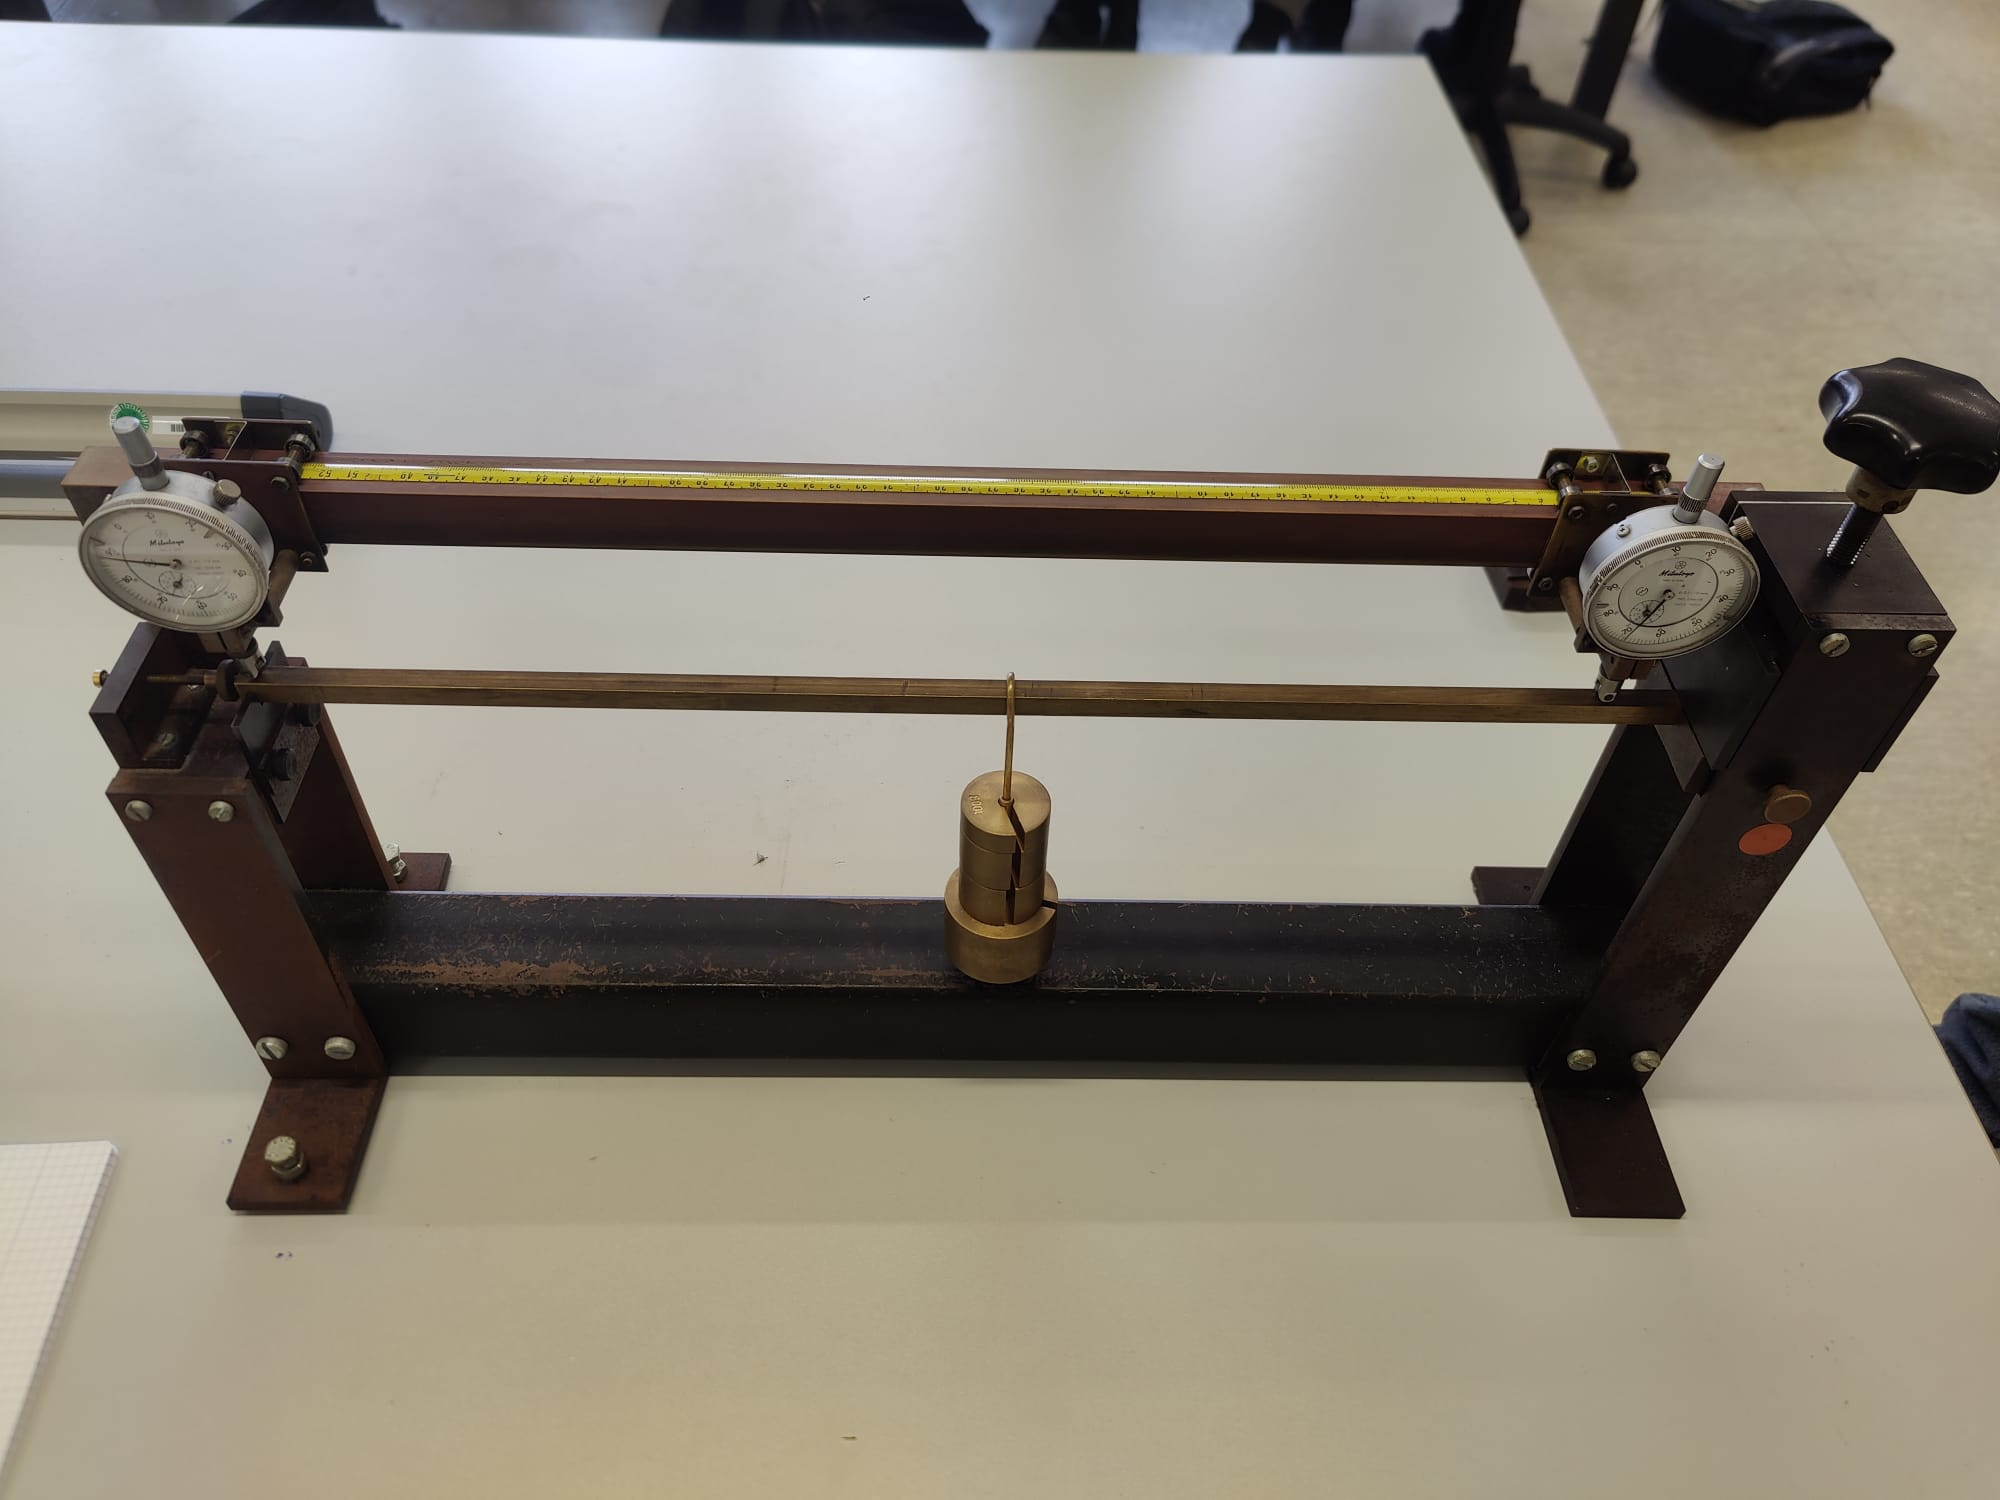
\includegraphics[width=\textwidth]{Bilder/bmG2.jpg}
        \caption{Beidseitige Einspannung des \\ eckigen Stabs mit Gewicht}
    \end{minipage}
\end{figure}
\subsection{Messung}
Bei der Messung werden jeweils 10 Werte aufgenommen. Dabei wird in regelmäßigen
Abständen die Uhr verschoben, sodass eine Auslenkung $D$ über ein breites 
Intervall festgehalten werden kann. Dabei besteht die Messung jeweils aus 2
Teilen, ein Mal mit und ein Mal ohne Gewicht.
